
\section{Introduction}
The prevalence of positioning devices has drastically boosted the scale of trajectory data collection. Instances include telemetry chips for animal herding histories, GPS devices for urban transportations and wearable devices for personal moving activities. These positional data are often time-stamped and can be viewed as trajectories. Data analysis on large-scale trajectory data can benefit a wide range of applications and services, including traffic planning, animal analysis, and social recommendations, just to name a few. CITATIONS FOR THE ABOVE APPLICATIONS.

An important task of data analysis on trajectories is to discover co-moving objects. Intuitively, a \emph{co-movement} pattern~\cite{li2013managing} consists of a set of objects that travel together for some duration. To formally define the pattern, the temporal dimension of trajectories is descritized into snapshots, where each snapshot contains the geographical information of all moving objects. Given a member size constraint $n$, a temporal constraint $k$, a \emph{co-movement} pattern finds a cluster of objects with at least size $n$ and close in spatial proximity for at least $k$ snapshots. Recently, there have been several works extending the basic pattern to incorporate more advanced temporal constraints. For instance, Jeung et al. proposed \emph{convoy} pattern, which requires the snapshots to be consecutive; Li et al. proposed \emph{swarm} pattern, which relaxes the consecutiveness of snapshots and Li et al. proposed \emph{platoon} pattern which imposed a \emph{minimum local length} on the snapshots. PLEASE BE MORE SPECIFIC FOR THE THREE PATTERNS. ALSO, ADD THE CITATIONS.


%We first provide a synthetic example to better illustrate these patterns in Figure~\ref{fig:related_work}, and the formal definitions are described in Section~\ref{sec:definition}.



Figure~\ref{fig:related_work} summarizes the differences among various co-movement patterns with an illustrative example. The temporal dimension is sliced into 5 snapshots. By setting $n=2$, the spatial clusters with at least $2$ objects are displayed with the same shape. Since \emph{Convoy} pattern requires the set of objects to be clustered for $k$ \emph{consecutive} snapshots, there results in only one such pattern ($\{o_3,o_4\}\{t_1,t_2,t_3\}$) when $k$ is set to $3$. \emph{Swarm} pattern relaxes the consecutiveness of duration, thus there are three patterns discovered. \emph{Platoon} pattern requires that each local consecutive duration needs to have at least certain length, which is indicated by an additional parameter $l$. When $l$ equals 2, there are two patterns discovered. Note that $\{o_6,o_7\}\{t_1,t_4,t_5\}$ is not included in the platoon pattern since $t_1$ is the local consecutive snapshot with duration 1, which is less than $l$. CAN WE SUPPORT THE GROUP AND FLOCK PATTERN? IF YES, WHY NOT PUT THEM IN THE FIGURE?

FOR THE FIGURE: 1) ENLARGE THE FONT SIZE IN THE FIGURE 2) WHY THERE IS NO $o_5$. 3) WHY OBJECTS IN DIFFERENT COLORS AND SHAPES ARE NOT CLEAR. YOU CAN REMOVE COLOR. 4) PUT THE OBJECTS BELONGING TO THE SAME CLUSTER IN THE SAME LINE.

\begin{figure} [t]
\center
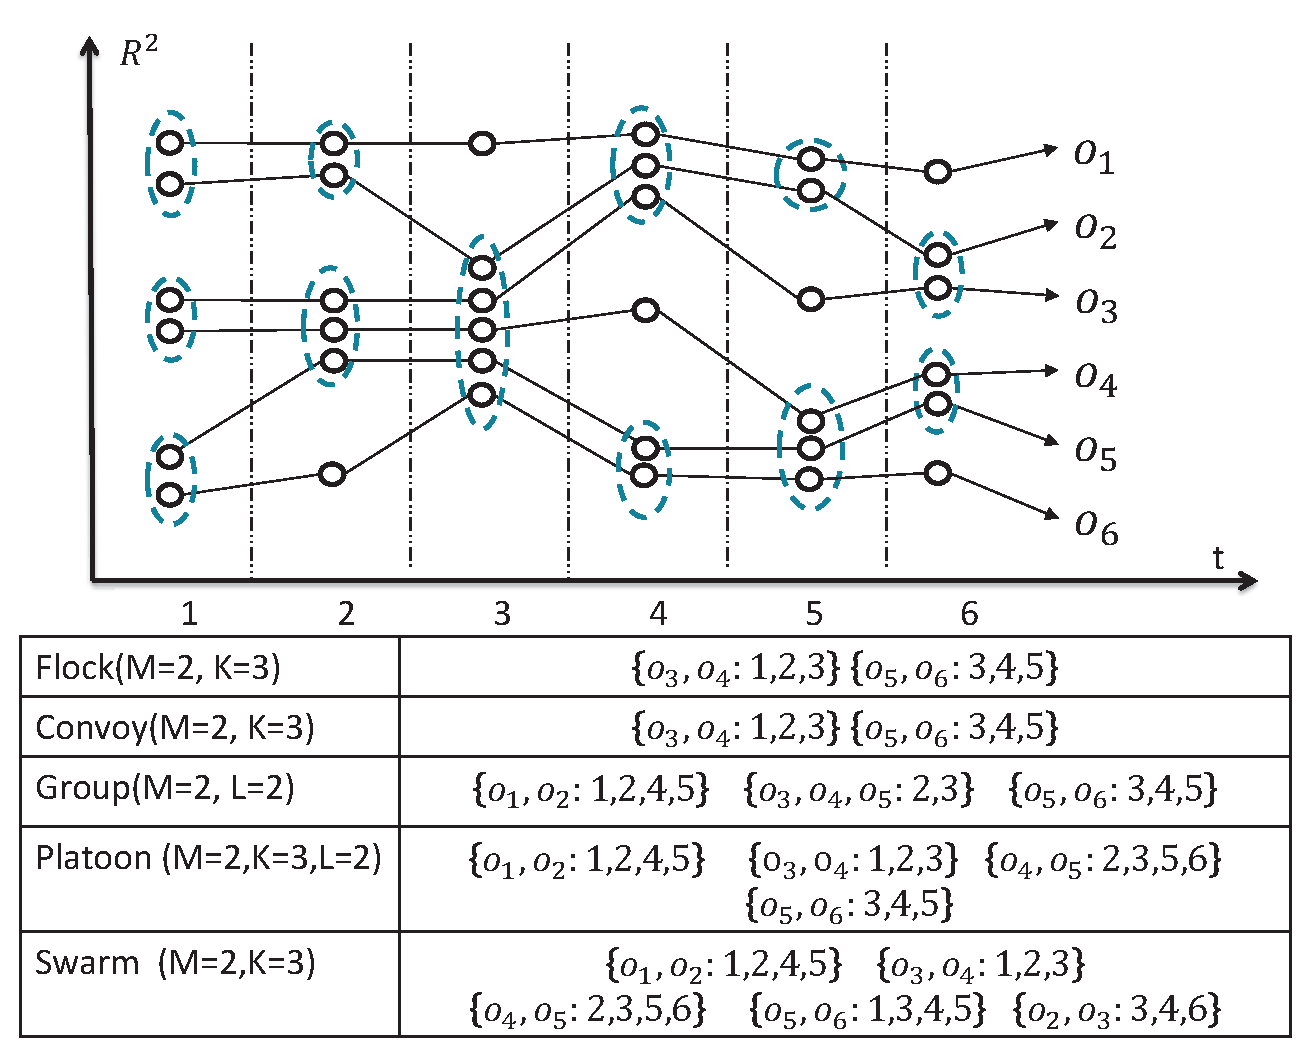
\includegraphics[width=0.5\textwidth]{related_work.eps}
\caption{Co-moving patterns in related works}
\label{fig:related_work}
\end{figure}

%We notice that, \emph{platoon} pattern is more general than \emph{convoy} and \emph{swarm}. This is because by setting appropriate $l$, \emph{platoon} can be reduced to \emph{convoy} and \emph{swarm} respectively~\cite{li2015platoon}. However, we observe that \emph{platoon} pattern is to loose on the temporal domain thus may result in less significant patterns. For example in Figure~\ref{fig:platoon_weakpoint}.



\begin{figure}[h]
\center
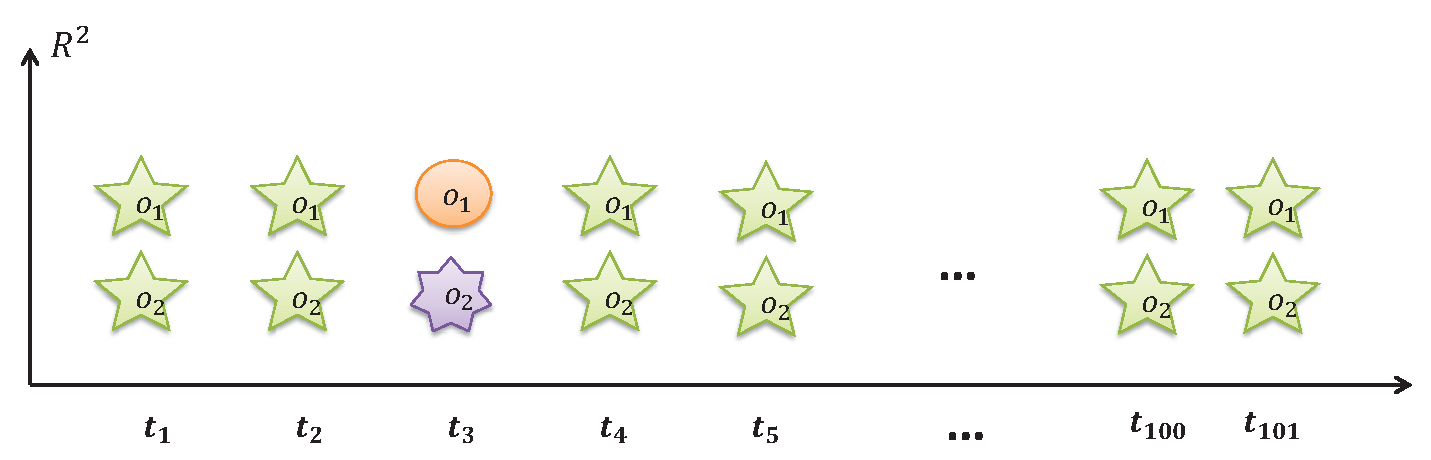
\includegraphics[width=0.5\textwidth]{platoon_weakpoint.eps}
\caption{Miss-pattern in platoon}
\label{fig:platoon_weakpoint}
\end{figure}

%In platoon, a pattern for $n=2,k=4,l=2$ could be $\{o_1, o_2\}\{t_1,t_2,t_4,t_5,t_{100},t_{101}\}$. However, the snapshots $t_{100}$ and $t_{101}$ is too far away from previous snapshots. Such two snapshots are in less relation with previous snapshots and thus should be removed from the pattern. Based on this observation, we defined a \emph{generalized co-moving} pattern (as in Section~\ref{sec:definition}) to provide a more fine granular control of the pattern. In \emph{generalized co-moving} pattern, a parameter $g$ is introduce the control the \emph{maximum gap} allowed between consecutive snapshots. By so doing our generalized co-moving pattern is more expressive and can represent all the existing co-moving patterns.

%In step with the advances in localization technologies, the growth in the volume of trajectory data is rapid. Traditional single-machine methods face severe scalability problem in handling large trajectory data. For example, as reported in~\cite{li2015platoon}, a \emph{Swarm} pattern takes around 100 seconds to discover for 100k trajectories. With upto billions of trajectories in nowadays datasets, such approaches apparently become unfeasible. To tackle this challenge, we propose a  paralleled solution for discovering \emph{generalized co-moving} patterns. We then deploy our idea on the modern MapReduce platform. As our experiments show, our solution achieves well load-balance and can process billions of trajectories in XXX seconds. Several optimizations are also designed to boost our solution to be orders of magnitudes faster than baseline algorithms.

%In practice, it is cumbersome to design tailed solutions to different types of co-movement pattern discovery. 

%In reality, it is cumbersome to design tailed solutions to support 
%generality and scalability

%In this paper, our primary objectives are solving two 
